\documentclass[main.tex]{subfiles}

\begin{document}

\section{Formule des moments et des interférences}
On considère les filtres:
{\huge
\begin{center}
  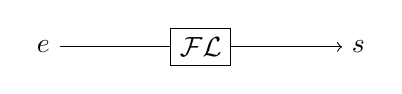
\begin{tikzpicture}
    \node (e) at (0,0) {$e$};
    \node[rectangle,draw] (f) at (2,0) {$\mathcal{FL}$};
    \node (s) at (4,0) {$s$};
    \draw[->] (e) -- (f) -- (s);
  \end{tikzpicture}
\end{center}}

On s'interesse aux filtre linéaires:

\begin{defin}
    \begin{itemize}
    \item Un fltre linéaire conservent la linéarité des systèmes auxquels il est appliqué.
    \item  Il est temps-invariant.
    \item et stationnaire.
    \end{itemize}
    On peux caractériser un filtre linéaire par:
    \begin{itemize}
    \item sa réponse impulsionnelle $h$
    \item sa réponse fréquentielle $H= TF[h]$
    \item sa fonction de transfert $H_{II}$.
    \end{itemize}
\end{defin}

\begin{prop}[Moyenne]
  \[
m_s = H(0) m_e
  \]
\end{prop}

Pour deux filtres on a :
\begin{center}
  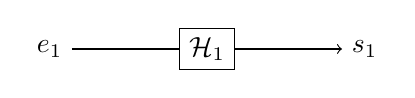
\begin{tikzpicture}
    \node (e) at (0,0) {$e_1$};
    \node[rectangle,draw] (f) at (2,0) {$\mathcal{H}_1$};
    \node (s) at (4,0) {$s_1$};
    \draw[->] (e) -- (f) -- (s);
  \end{tikzpicture}\\[1.5em]
  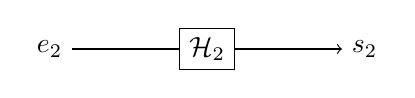
\begin{tikzpicture}
    \node (e) at (0,0) {$e_2$};
    \node[rectangle,draw] (f) at (2,0) {$\mathcal{H}_2$};
    \node (s) at (4,0) {$s_2$};
    \draw[->] (e) -- (f) -- (s);
  \end{tikzpicture}
\end{center}

\begin{prop}[Formule des interférences]

  \[
\Gamma_{s_1,s_2}(f)=H_1(f)\cdot H_2(f)^*\cdot \Gamma_{e_1,e_2}(f)
  \]
\end{prop}
\section{Application}
\subsection{Blanchiement d'un signal}

Pour générer un bruit blanc $s(t)$ on veux  :
\[
  \Gamma_0 = |H(f)|^2\Gamma_{ee}(f)\implies |H(f)|^2 = \frac{\Gamma_0}{\Gamma_{ee}(f)}
\]


\subsection{Identification d'un filtre linéaire}

On applique en entrée un bruit blanc tel que $\Gamma_{ee}(f)=\Gamma_0$.
Alors:
\[
  \Gamma_{se}=H(f)\Gamma_e(f) \implies H(f)=\frac{\Gamma_{se}(f)}{\Gamma_0} \propto \text{intercorrélation entrée sortie}
\]


\subsection{Signaux ARMA}

On peux utilise un Filtre Linéaire (FL) pour définir un Signal Aléatoire.
(SA).
Le SA sera la sortie d'un filtre dynamique (Fonction de transfert rationnel ,stable ,causal) excité par un bruit blanc.


\subsubsection{AR : autoregressif}


\[
  \boxed{
    H_{II}(z) = \frac{1}{D(z)}=\frac{1}{1-\sum_{i=1}^qa_iz^{-i}}
  }
\]
Alors on aura en sortie du filtre:
\[
  s_k= e_k + \sum_{i=1}^qa_is_{k-i}
\]

on parle aussi de filtre \og tout pôle\fg{}

\subsubsection{MA : Moyenne ajustée}

\[
  \boxed{
    H_{II}(z) = N(z)= 1+\sum_{i=1}^qb_iz^{-i}
  }
\]

Alors on aura en sortie du filtre:
\[
  s_k= e_k + \sum_{i=1}^qb_ie_{k-i}
\]


\subsubsection{ARMA}

\[
H_{II}(z) = \frac{N(z)}{D(z)}
\]

On connait alors $\Gamma_{ss}$ et le modèle AR. (Équation de Yule WAlker, cf TP2)
\subsection{Signaux AR : illustration}


pour une entrée en bruit blanc , les poles proches du cercle unités sont dominant
(approche géométrique , joli dessin)



\subsection{Filtre Adapté (FA)}

\paragraph{Contexte} Problème de transmission numérique (tout ou rien) d'un signal déterministe, connu avec bruit additif.
\paragraph{Objectif} déterminer le meilleur traitement linéaire pour décider de la présence ou  non d'un signal.

Exemple en TD
\paragraph{Méthode} :Maximiser le RSB à l'instant de décision : avec $|s_{n_0}^f|^2$ puissance instantanée à l'instant de décision.
\[
  \boxed{
    \frac{|s_{n_0}^f|^2}{E[|b_n^f|^2]}
  }
\]
\begin{prop}[Application au bruit blanc]
  \begin{align*}
    E[|b_n^f|^2] &=\int_{-\frac{1}{2}}^{\frac{1}{2}} |H(f)|^2\Gamma_{bb}(f)df = \Gamma_0\int_{-\frac{1}{2}}^{\frac{1}{2}} |H(f)|^2df \\
|S_{n_0}^f|^2 &=  \left| \int_{-\frac{1}{2}}^{\frac{1}{2}} |H(f)|^2 S(f) e^{j2\pi n_0f}df\right| \leq \int_{-\frac{1}{2}}^{\frac{1}{2}} |H(f)|^2df \int_{-\frac{1}{2}}^{\frac{1}{2}} |S(f)|^2df
  \end{align*}

  On a égalité si $H(f)\propto S^{*}(f)e^{-j2\pi n_0f} \iff h_n \propto s_{n_0-n}^f$

LA RI du filtre est donc
  \begin{itemize}
  \item un retour temporel
  \item translaté autour de l'instant de décision (attention a la causalité)
  \item conjugué.
  \end{itemize}
\end{prop}


\paragraph{Remarque}
\begin{itemize}
\item Le FA peut être non causal, la RI est alors tronqué et le filtre
  sous-optimal.
\item Le FA est un corrélateur (d'énergie), l'objectif n'est pas de restituer le signal utile mais d'avoir le meilleur RSB à l'instant de décision.
\end{itemize}

\end{document}
